\documentclass{edm_article}
\usepackage{hyperref}
\hypersetup{
    colorlinks=true,
    linkcolor=cyan,
    filecolor=magenta,      
    urlcolor=magenta,
    pdftitle={Overleaf Example},
    pdfpagemode=FullScreen,
    }
\begin{document}

\title{Transport Phenomena in Drug Resistance in the Treatment of Acute Myeloid Leukemia}

\numberofauthors{1}
\author{
Yuqi X.\\
Nov 18th, 2021\\
       \affaddr{University of British Columbia}
}

\maketitle

\begin{abstract}
This paper provides a mathematical model for drug resistance with respect to transport phenomena in acute myeloid leukemia. We investigate drug efflux due to the over-expression of P-glycoprotein, and its effect on drug resistance in chemotherapy. 
\end{abstract}

%\keywords{Transport phenomena, drug resistance, drug efflux, Pgp} % Replace with your own 3-5 keywords

\section{Introduction}
Acute myeloid leukemia (AML) is a common type of cancer caused by the growth of abnormal cells in the bone marrow and blood, stunting the growth of normal blood cells.\cite{AML} Treatment of AML includes the use of anticancer drugs released into the bloodstream to destroy or control cancer cells. However, the development of drug resistance has been observed especially during relapse. Several mechanisms can contribute to the development of drug resistance, including failure of cancer cells to go through apoptosis, and low steady-state concentration of drug reaching the intracellular target.\cite{resistance}

P-glycoprotein (Pgp) is a transporter that acts as a pump to export chemicals from cells, it's usually located on the plasma membrane, but it can also be found intracellularly. Over-expression of Pgp is found in a lot of cancer cells including in AML.\cite{Pgp} This phenomena causes high drug efflux and consequently decreases steady-state drug concentration at the target. This paper models how intracellular Pgp concentration influences drug resistance in the treatment of AML. We approach this by a two-step DE analysis 1) a set of differential equations modelling sensitive cell mass and resistant cell mass; 2) diffusion equation in spherical coordinates with a loss function contributed by Pgp expression.

The model we obtain may shed insights on how Pgp expression in cells influences steady state concentration of drug molecules undergoing single cell diffusion, and the interaction between sensitive and resistant cell types. Our model links microscopic diffusion with cell destruction and development of resistance at a macroscopic level. 

\section{Intracellular Diffusion}
\textbf{Single cell diffusion} We considering the following diffusion equation in the spherical coordinate, assuming radial symmetry, with an additional loss term contributed to by Pgp expression.
\begin{align*}
    \frac{\partial u}{\partial t} &= \frac{D}{r^2}\frac{\partial}{\partial r}(r^2\frac{\partial u}{\partial r}) - L
\end{align*}
Here $u$ is the concentration of the drug, it is dependent on time $t$ and radius $r$. $L$ is the loss term, representing drug loss due to active Pgp transporters in the cell. We consider the following boundary conditions.

\textbf{Boundary conditions}
\begin{align*}
    u(r = b, t = 0) &= c\\
    u(r < b, t = 0) &= 0\\
    \frac{\partial u}{\partial t}(r = a, t) &= 0
\end{align*}
Here $b$ is the radius at cell membranes, $a$ is the radius at the nucleus (target of the drug). We assume that the a constant concentration of drug reaches the cell membrane at time zero, when there is zero drug concentration in other parts of the cell. When the drug reaches the nucleus of the cell, it gets absorbed, and the cell either goes through apoptosis or builds up resistance depending on the concentration of drug that reaches the cell.

\textbf{Loss Term} $L$ is the loss term associated with Pgp expression. A simplistic approach to model this term is to assume that it is proportional to the intracellular concentration of Pgp. But this would fail when the concentration of the drug becomes low. Nevertheless we assume $L$ is constant for the sake of calculating a general solution. A more reasonable model would state that $L$ is proportional to the product of concentration of Pgp and the concentration of the drug. A more advanced model may include the transport and diffusion of Pgp and the drug.
\begin{align*}
    L = -\frac{du}{dt} = -k_{out}\cdot uP + k_{off}\cdot B
\end{align*}
Here $u$ is the concentration of the drug, $P$ is the concentration of Pgp, and $B$ is the concentration of the bounded complex.

\textbf{General solution} Using separation of variables, we take
\begin{align*}
    &u(r,t) = R(r)T(t)\\
    &R(r)T'(t) = DT(t)\frac{1}{r^2}\partial_r(r^2R'(r))\\
    &\frac{T'(t)}{T(t)} = -\lambda\\
    &T(t) = f_0e^{-\lambda t}\\
\end{align*}
This gives us the time-dependent part of the concentration, now on to the radial part.
\begin{align*}
    &D\frac{1}{r^2}\partial_r(r^2R'(r)) = -\lambda R(r)\\
    &R(r) = c_1 \frac{e^{-ir\sqrt{\lambda/D}}}{r} + c_2 \frac{e^{-ir\sqrt{\lambda/D}}}{r}
\end{align*}
which yields the general solution
\begin{align*}
    u(r,t) = (c_1 \frac{e^{-ir\sqrt{\lambda/D}}}{r} + c_2 \frac{e^{-ir\sqrt{\lambda/D}}}{r})f_0e^{-\lambda t}
\end{align*}
We are interested in the drug concentration profile at the nucleus over time, and the overall drugs received at each dose, these are respectively
\begin{align*}
    &u(r = a, t) = (c_1 \frac{e^{-ia\sqrt{\lambda/D}}}{a} + c_2 \frac{e^{-ia\sqrt{\lambda/D}}}{a})f_0e^{-\lambda t}\\
    &u_{Total}= (c_1 \frac{e^{-ia\sqrt{\lambda/D}}}{a} + c_2 \frac{e^{-ia\sqrt{\lambda/D}}}{a})\int_{t = 0}^{t_f}f_0e^{-\lambda t}\\
\end{align*}

\section{Heterogeneous Tumor Model}
\textbf{Modelling sensitive vs. resistance cell types} We consider the following set of differential equations for sensitive cell mass and resistant cell mass.
\begin{align*}
    \frac{dx}{dt} &= (r_1 - d_1(t))x\\
    \frac{dy}{dt} &= bd_1(t)x + (r_2-d_2(t))y
\end{align*}
Here $x$ is the sensitive cell mass with low Pgp expression and requires lower dosage at nucleus to go through apoptosis, $y$ is the resistant cell mass with high Pgp expression and requires higher dosage to go through apoptosis. $r_1, r_2$ are the cell growth rate for $x,y$ respectively, and $d_1(t), d_2(t)$ are time dependent periodic functions for cell loss related to Pgp expression. But in essence these two functions model the transport of drug to the nucleus over different dosages. $b$ is the induction coefficient which is a real number in the interval [0,1]. This constant serves the purpose of identifying how much of the sensitive cell loss happened through apoptosis and how much of it happened through sensitive cells converting to resistant cells. Intuitively, $b = 1$ indicates that no cells ever go through apoptosis when targeted by chemotherapy drugs, and $b = 0$ indicates that there is no build-up of drug resistance. 

\textbf{From microscopic diffusion to macroscopic destruction} The periodic functions $d_1(t), d_2(t)$ models the rate of destruction over time. The period of these functions is $\tau$, the time taken from drugs being released at cell membranes to when all drugs are being absorbed at the nucleus or carried out through efflux over one dosage. Repeated dosages are expressed through repeating periods of our destruction functions. Ideally, these functions take information from single cell diffusion and use that to determine cell destruction. 

One way to link these is by the following mechanism: For sensitive cell types, if $u_{Total} \leq k_1$, cell builds up resistance, if $u_{Total} > k_1$, cell goes through apoptosis. For resistant cell types, if $u_{Total} > k_2$, cell goes through apoptosis. $k_1, k_2$ are threshold concentration values and intuitively $k_2 > k_1$, as resistant cells needs higher concentration of drugs in order to go through apoptosis. 

For our purposes, we will assume the destruction rates are constant, or that it follows a bell curve distribution. 
\begin{align*}
    f(x) = \frac{1}{\sigma\sqrt{2\pi}}e^{-0.5(\frac{x-\mu}{\sigma})^2}
\end{align*}

\section{Numerical Approximation}
The more advanced version of our single cell diffusion model is not solvable analytically. We consider a forward time centered space scheme to approximate our results numerically. 

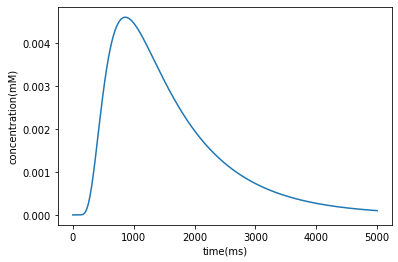
\includegraphics[scale = 0.6]{sensitive.png}\\
\textbf{Figure 1: Concentration profile at nucleus over time for sensitive cell type}

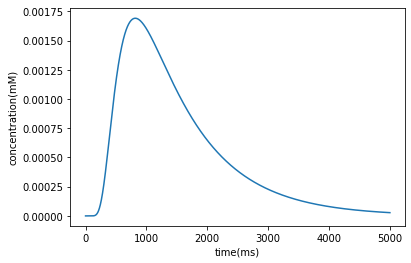
\includegraphics[scale = 0.6]{resistant.png}\\
\textbf{Figure 2: Concentration profile at nucleus over time for resistant cell type}

We model the cell conversion model with the destruction function as a constant and as a bell curve respectively, the following figures are the results. The red line shows the growth of sensitive cell and the green line shows the growth of resistant cells.

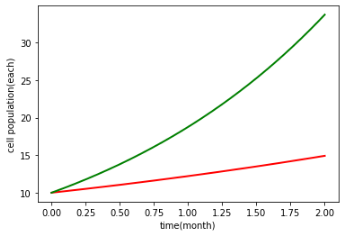
\includegraphics[scale = 0.6]{constant.png}\\
\textbf{Figure 3: Cell type conversion with constant destruction rates}

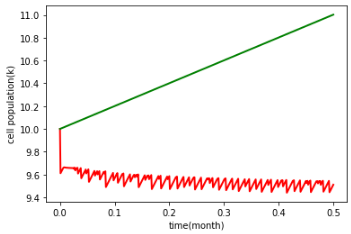
\includegraphics[scale = 0.6]{bell.png}\\
\textbf{Figure 4: Cell type conversion with varying destruction rates}

\section{Conclusions}
Our model shows that high Pgp concentration leads to low drug concentration received at the nucleus, resulting in drug resistant. We also observe that over time, resistant cells grow faster than sensitive cells. Sensitive cells have the potential to be destroyed or controlled over the course of treatment if they don't build up resistance.

\textbf{Pgp expression and drug concentration profile at nucleus} By numerical approximation, we find that about 75.1\% of drugs released at cell membrane reaches the nucleus in sensitive cells, and 26.3\% of drugs released at cell membrane reaches the nucleus in resistant cells. Figure 1, 2 shows that the concentration profiles at nucleus over time follows the same distribution. Concentration peaked at about 0.0044mM for sensitive cells and 0.00169mM for resistant cells. 

\textbf{Sensitive vs. resistant cell population} We observe that in the case of constant destruction rates, both cell populations grow exponentially. Resistant cells tripled in their population over 2 months, while sensitive cell populations grew about 1.5 its original size. In the case of varying destruction rates modelled by a bell curve, we observe that resistant cell population grows exponentially where as the sensitive cell population is controlled and decreasing overall. 

\textbf{Clinical implications} We make two clinical implications from our model. 1) Since high Pgp concentration contributes to drug resistance, Pgp inhibitors may be administered along with chemotherapy drugs to reduce drug efflux. 2) It is important to control dosages of chemotherapy drugs, in order to suppress both cell types without introducing drug resistance which will stunt the treatment progress. 

\section{Evaluation and Future Work}
Mechanisms for drug resistance is extremely complex, this paper chose to focus on one aspect of it -- namely intracellular Pgp concentration. While our model produced desirable results that aligns with biological intuitions, there are several limitations that we discuss in this section.

\textbf{Pgp transport and reaction} In our numerical model, we did not take account of Pgp transport in cells. We also ignored the intracellular distribution and the transport rate of Pgp. 

\textbf{Boundary conditions} In our boundary condition we assumed that the blood will carry a constant amount of drugs to the membrane at time zero at the beginning of each dosage, this is not accurate. In future work, it may benefit us to consider intercellular transport and diffusion, where drug concentration at cell membrane is treated as a continuous function instead of a discrete value. 

\textbf{From microscopic to macroscopic views} Ideally, we'd like the cell type conversion model to take information from what happens in single cell diffusion. This is not well-developed in our current model. In future work, we'd like to look at mechanisms that links drug resistance from a microscopic to a macroscopic view. 

\textbf{Charge of the drug molecule} The charge on the drug molecules, in other words how nucleophilic the molecules are, influences the rate of transport towards the nucleus. This may limit the rate of drug efflux and therefore increase the percentage of drug molecules reaching the nucleus. In future work, this should be taken into account. 

%ACKNOWLEDGMENTS are optional
\section{Acknowledgments}
The author would like to acknowledge that this research was done on the traditional, ancestral, and unceded territory of the Musqueam people.

%
% The following two commands are all you need in the
% initial runs of your .tex file to
% produce the bibliography for the citations in your paper.
\bibliographystyle{abbrv}
\bibliography{sigproc}

\begin{appendix}
The python code and original Tex file for the project can be accessed at \href{https://github.com/Yuqi-eng/Drug-Resistance-in-AML}{this github repo} or \url{https://github.com/Yuqi-eng/Drug-Resistance-in-AML}.
\end{appendix}
\end{document}
